\documentclass[12pt]{article}

\usepackage[a5paper, landscape, margin=10mm]{geometry}
\usepackage{enumitem}
\usepackage{amsmath}
\usepackage{amssymb}
\usepackage{amsfonts}
\usepackage{placeins}
\usepackage{graphicx}
\usepackage{listings}
\usepackage{caption}
\usepackage{colortbl}
\usepackage[parfill]{parskip}
\usepackage[mathscr]{euscript}
\usepackage[usenames,dvipsnames,svgnames,table,hyperref]{xcolor}
\usepackage[hidelinks]{hyperref}
\usepackage{fontspec}
\usepackage{mdframed}

\setsansfont{FreeSans}
\setmonofont{Ubuntu Mono}
\renewcommand{\familydefault}{\sfdefault}

\hyphenation{WebGL}

\definecolor{webColor}{RGB}{0, 108, 174}
\newcommand{\web}[1]{{\color{webColor} \small \url{#1}}}
\newcommand{\webText}[2]{{\color{webColor} \href{#2}{#1}}}
\newcommand{\email}[2]{{\small \color{webColor} \textsf{\href{mailto:#1@#2}{#1[at]#2}}}}
\definecolor{titleColor}{RGB}{179, 0, 149}
\newcommand{\myTitle}[1]{{\large \color{titleColor} \hspace{-4mm} \textbf{\textsf{#1}}}}
\definecolor{subColor}{RGB}{179, 0, 149}
\newcommand{\mySub}[1]{\textsf{\color{subColor}#1}}
\definecolor{keyColor}{RGB}{170, 149, 0}
\newcommand{\myKey}[1]{\textbf{\color{keyColor}#1}}

\definecolor{redBoxFg}{RGB}{255, 0, 0}
\definecolor{redBoxBg}{RGB}{255, 218, 232}
\newcommand{\redBox}[1]{{\color{redBoxFg}\colorbox{redBoxBg}{#1}}}
\definecolor{yellowBoxFg}{RGB}{0, 0, 0}
\definecolor{yellowBoxBg}{RGB}{255, 232, 0}
\newcommand{\yellowBox}[1]{{\color{yellowBoxFg}\colorbox{yellowBoxBg}{#1}}}
\definecolor{greenBoxFg}{RGB}{0, 0, 0}
\definecolor{greenBoxBg}{RGB}{134, 210, 153}
\newcommand{\greenBox}[1]{{\color{greenBoxFg}\colorbox{greenBoxBg}{#1}}}
\definecolor{blueBoxFg}{RGB}{0, 0, 255}
\definecolor{blueBoxBg}{RGB}{218, 232, 255}
\newcommand{\blueBox}[1]{{\color{blueBoxFg}\colorbox{blueBoxBg}{#1}}}
\definecolor{violetBoxFg}{RGB}{0, 0, 0}
\definecolor{violetBoxBg}{RGB}{218, 204, 255}
\newcommand{\violetBox}[1]{{\color{violetBoxFg}\colorbox{violetBoxBg}{#1}}}

\mdfdefinestyle{MyFrame}{%
    linecolor=black,
    outerlinewidth=0pt,
    linewidth=0pt,
    innertopmargin=2.7pt,
    innerbottommargin=0pt,
    innerrightmargin=0pt,
    innerleftmargin=0pt,
        leftmargin = 0pt,
        rightmargin = 0pt}

\definecolor{lightttColor}{RGB}{69, 69, 80}
\newcommand{\lighttt}[1]{{\color{lightttColor}\texttt{#1}}}

\renewcommand*\labelenumi{(\theenumi)}
\renewcommand*{\theenumii}{\roman{enumii}}
\renewcommand*\labelenumii{\theenumii.}

\newcommand{\fixminipage}{\raggedright \setlength{\parskip}{0.3\baselineskip}}
\newcommand{\codeminipage}{\raggedright \setlength{\parskip}{0\baselineskip}}
\sloppy
\pagenumbering{gobble}


\begin{document}

\tikzstyle{smallnode} = [rectangle, minimum width=1.25cm, minimum height=1cm, text centered, text width=1.25cm, draw=black, fill=white]
\tikzstyle{smallishnode} = [rectangle, minimum width=2cm, minimum height=1cm, text centered, text width=2cm, draw=black, fill=white]
\tikzstyle{normalnode} = [rectangle, minimum width=3cm, minimum height=1cm, text centered, text width=3cm, draw=black, fill=white]
\tikzstyle{widenode} = [rectangle, minimum width=62mm, minimum height=8mm, text centered, text width=62mm, draw=black, fill=white]
\tikzstyle{bignode} = [rectangle, minimum width=3.5cm, minimum height=2cm, text centered, text width=3cm, draw=black, fill=white]
\tikzstyle{smemnode} = [rectangle, minimum width=3cm, minimum height=1cm, text centered, text width=3cm, draw=keyColorB, fill=white]
\tikzstyle{gmemnode} = [rectangle, minimum width=3cm, minimum height=1cm, text centered, text width=3cm, draw=keyColorA, fill=white]
\tikzstyle{smallishsmemnode} = [rectangle, minimum width=2cm, minimum height=1cm, text centered, text width=2cm, draw=keyColorB, fill=white]
\tikzstyle{arrow} = [thick,->,>=stealth]
\tikzstyle{line} = [thick]

{ \LARGE Exo Dev 2025-05-06 } \hfill { \LARGE \textbf{\textsf{Spork: GEMM Samples}}}

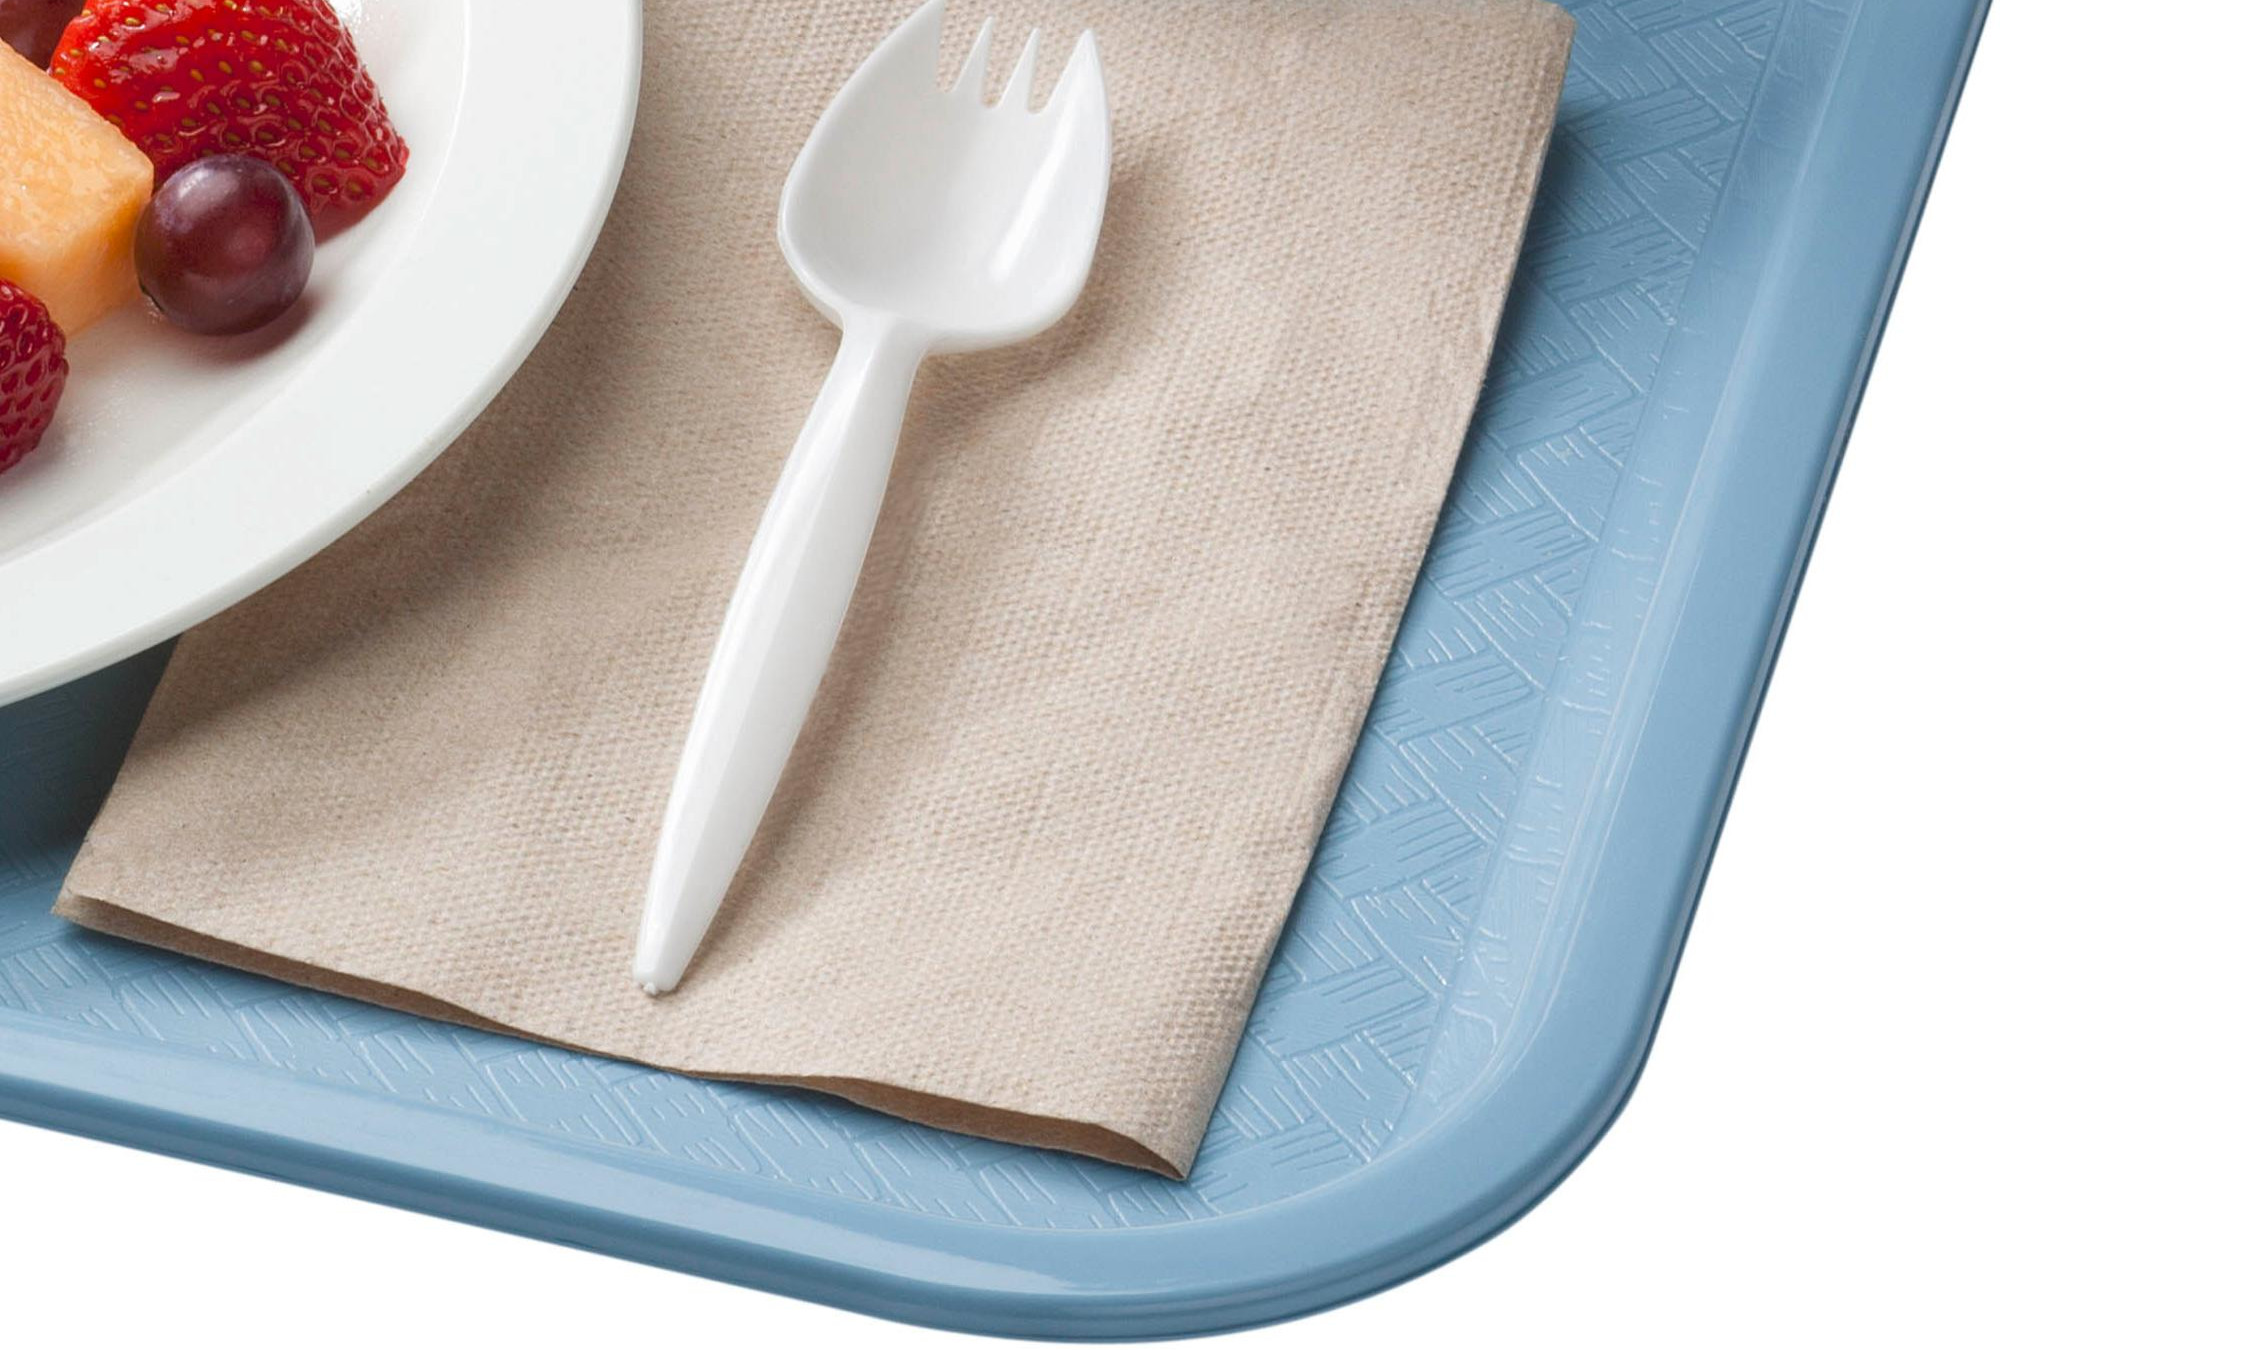
\includegraphics[width=\linewidth]{usda_spork.jpg}

\newpage
\myTitle{Intro 0}

\input{gemms_tex/intro.0.tex}
\newpage
\myTitle{Intro 1}

\input{gemms_tex/intro.1.tex}

\newpage
\myTitle{Intro 2}

\input{gemms_tex/intro.2.tex}

\newpage
\myTitle{Par}

\input{gemms_tex/par.0.tex}

\newpage
\myTitle{Tile 0}

\input{gemms_tex/tile.0.tex}
\newpage
\myTitle{Tile 1}

\input{gemms_tex/tile.1.tex}

\newpage
\myTitle{Tile 2}

\input{gemms_tex/tile.2.tex}

\newpage
\myTitle{GMEM}

\input{gemms_tex/gmem_remark.0.tex}

\newpage
\myTitle{SMEM Alloc}

\input{gemms_tex/smem_alloc.0.tex}

\newpage
\myTitle{Broken SMEM 0}

\input{gemms_tex/broken_smem.0.tex}

\newpage
\myTitle{Broken SMEM 1}

\input{gemms_tex/broken_smem.1.tex}

\newpage
\myTitle{Broken SMEM 2}

\input{gemms_tex/broken_smem.2.tex}

\newpage
\myTitle{Distributed Memory 0}

\input{gemms_tex/dmem.0.tex}

\newpage
\myTitle{Distributed Memory 1}

\input{gemms_tex/dmem.1.tex}

\newpage
\myTitle{Distributed Memory 2}

\input{gemms_tex/dmem.2.tex}

\newpage
\myTitle{Distributed Memory 3}

\input{gemms_tex/dmem.3.tex}

\newpage
\myTitle{Distributed Memory 4}

\input{gemms_tex/dmem.4.tex}
\newpage
\myTitle{Distributed Memory 5}

\begin{minipage}[t]{0.48\textwidth}\fixminipage
\mySub{Before}

\input{gemms_tex/dmem_before.0.tex}
\end{minipage}
\hfill
\begin{minipage}[t]{0.48\textwidth}\fixminipage
\mySub{After}

\input{gemms_tex/dmem_after.0.tex}

\vspace{4mm}
Distributed dimensions (\blacktt{f32[\greenBox{16}, \violetBox{16}, ...]}) are elided in the generated C++ code.
\end{minipage}

\newpage
\myTitle{Working SMEM Example 0}

\input{gemms_tex/working_smem.0.tex}

\newpage
\myTitle{Working SMEM Example 1}

\input{gemms_tex/working_smem.1.tex}
\newpage
\myTitle{Working SMEM Example 2}

\input{gemms_tex/working_smem.2.tex}

\newpage
\myTitle{Ring Buffer 0}

\input{gemms_tex/ring.0.tex}

\newpage
\myTitle{Ring Buffer 1}

\input{gemms_tex/ring.1.tex}

\newpage
\myTitle{Ring Buffer 2}

\input{gemms_tex/ring.2.tex}

\newpage
\myTitle{Before TMA}

\input{gemms_tex/ring.3.tex}

\newpage
\myTitle{Prep TMA 0}

\input{gemms_tex/prep_tma.0.tex}

\newpage
\myTitle{Prep TMA 1}

\input{gemms_tex/prep_tma.1.tex}

\newpage
\myTitle{TMA 0}

\input{gemms_tex/tma.0.tex}

\newpage
\myTitle{TMA 1}

\input{gemms_tex/tma.1.tex}

\newpage
\myTitle{TMA 2}

\input{gemms_tex/tma.2.tex}

\newpage
\myTitle{TMA 3}

\input{gemms_tex/tma.3.tex}

\newpage
\myTitle{TMA Forward Synchronization}

\input{gemms_tex/prep_tma.2.tex}

\newpage
\myTitle{TMA Reverse Synchronization}

\input{gemms_tex/prep_tma.3.tex}

\newpage
\myTitle{Next Steps: Tensor Cores}

\input{gemms_tex/wgmma.0.tex}


\end{document}
